% !TEX TS-program = pdflatex
% !TEX encoding = UTF-8 Unicode
\documentclass[12pt,
    driverfallback=dvipdfm,
 %   openright,
 	openany,
    a4paper,
 %   parskip=half,   
    toc=bibliography,
    twoside,
    numbers=noenddot]{book}              % Book class in 11 points
    \usepackage[usenames,dvipsnames,showerrors]{xcolor}
    \usepackage[
    driverfallback=dvipdfm,
    colorlinks,
    linkcolor=blue,
    citecolor=blue,
    urlcolor=black,
    bookmarks=true
    ]{hyperref}
    
\usepackage{algorithmic}
%\usepackage{algorithmicx}
%\usepackage[ruled]{algorithm}
%\usepackage{algpseudocode}

\usepackage{logicproof}
\usepackage{fancyhdr}
%\usepackage{mathptmx}
\usepackage{makeidx}
\makeindex



\usepackage{float}
\floatstyle{ruled}
\newfloat{problem}{thp}{lop}
\floatname{problem}{Problem}
\usepackage{enumitem}
\usepackage{multicol}
\usepackage[rightcaption]{sidecap}
 
%\usepackage{graphicx} %package to manage images
%\graphicspath{ {images/} }
%\usepackage{fullpage}
    
%\raggedright                            % do not right justify


\title{\bf Linear Programming}    % Supply information
\author{Sreejith A. V. (sreejithav@iitgoa.ac.in)}              %   for the title page.
\date{IIT Goa, seminar series}                           %   Use current date. 
%\usepackage{mwe}
%\usepackage{xcolor}
%\usepackage[markcase=noupper]{scrlayer-scrpage}

\pagestyle{fancy}
\fancyhf{}
\fancyhead[LE]{\leftmark}
\fancyhead[RO]{\rightmark}
%\fancyhead[RE,LO]{Guides and tutorials}
\fancyhead[LO]{~}
\fancyhead[RE]{~}
%\fancyfoot[CE,CO]{\leftmark}
\fancyfoot[LE,RO]{\thepage}
 
%\renewcommand{\headrulewidth}{1pt}
%\renewcommand{\footrulewidth}{1pt}
\renewcommand{\chaptermark}[1]{\markboth{\thechapter.\ #1}{}}

%\ohead{}% clear the outer head
%\addtokomafont{pagehead}{\sffamily}
%\addtokomafont{pagefoot}{\tiny}% Making the foot extra tiny to demonstrate
%\addtokomafont{pagenumber}{\normalsize}% that the page number can be controlled on its own. 
%\ofoot*{\pagemark}% the pagenumber in the outer part of the foot, also on plain pages
%\ifoot*{Sreejith\\sreejithav@iitgoa.ac.in}% Name and title beneath each other in the inner part of the foot
%\setlength{\footheight}{24.0pt}

%\documentclass[UKenglish,a4paper,12pt]{article} % use larger type;
%\usepackage[utf8]{inputenc} % set input encoding (not needed with XeLaTeX)
%\usepackage[T1]{fontenc}
%\usepackage{lmodern}

% Author macros::begin %%%%%%%%%%%%%%%%%%%%%%%%%%%%%%%%%%%%%%%%%%%%%%%%
%\title{\mathversion{bold}2. Propositional Logic}
%\author{A. V. Sreejith (IIT Goa)}
%\date{~}

\newcommand\tab[1][1cm]{\hspace*{#1}}

%%% PACKAGES
\usepackage{tikz}
\usetikzlibrary{shapes,arrows, positioning}
\usepackage{algorithm,algorithmic}% http://ctan.org/pkg/algorithms


\usepackage{amssymb,amsmath,amsthm}
\usepackage{bussproofs}
\usepackage{mdframed} \usepackage[dvipsnames]{xcolor}

\usepackage{caption}
\usepackage{subcaption}
\usepackage{xspace}

\usepackage{float}
\restylefloat{table}


\newtheorem{theorem}{Theorem}[chapter]
\newtheorem{corollary}{Corollary}[chapter]
\newtheorem{definition}{Definition}[chapter]
\newtheorem{exercise}{Exercise}[chapter]
\newtheorem{example}{Example}[chapter]
\newtheorem{puzzle}{Puzzle}[chapter]
\newtheorem*{solution}{Solution}

\newtheorem{innercustomgeneric}{\customgenericname}
\providecommand{\customgenericname}{}
\newcommand{\newcustomtheorem}[2]{%
  \newenvironment{#1}[1]
  {%
   \renewcommand\customgenericname{#2}%
   \renewcommand\theinnercustomgeneric{##1}%
   \innercustomgeneric
  }
  {\endinnercustomgeneric}
}

\newcustomtheorem{customthm}{Theorem}
\newcustomtheorem{customlemma}{Lemma}
\newtheorem{lemma}[theorem]{Lemma}
\newtheorem{claim}[theorem]{Claim}

\definecolor{light-gray}{gray}{0.95}
\newcommand{\odd}{{\normalfont{Odd}}\xspace}
\newcommand{\even}{{\normalfont{Even}}\xspace}
\newcommand{\finocc}[1]{\mathrm{FIN}(#1)\xspace}
\newcommand{\infocc}[1]{\mathrm{INF}(#1)\xspace}

\newcommand{\Nat}{\mathbb{N}}
\newcommand{\Reals}{\mathbb{R}}
\newcommand{\Rn}{\Reals^n}
\newcommand{\closedset}[2]{[#1, #2]}

\begin{document}
%\frontmatter                            % only in book class (roman page #s)
%\maketitle                              % Print title page.
%\tableofcontents                        % Print table of contents
%\mainmatter                             % only in book class (arabic page #s)
\renewcommand{\vec}[1]{\mathbf #1}
\newcommand{\mat}[1]{{\mathbb #1}}
\newcommand{\trans}[1]{{#1}^{\mathsf{T}}}
\newcommand{\rowvec}[1]{\trans{\vec {#1}}}
\newcommand{\dotprod}[2]{\rowvec{#1}  \vec{#2}}
\newcommand{\minimize}{\mathtt{minimize}}
\newcommand{\maximize}{\mathtt{maximize}}

\newcommand{\Imatrix}{\mat{I}}
\newcommand{\cspace}[1]{C(\mat #1)}
\newcommand{\defs}{::=}
\newcommand{\BFS}{\ensuremath{\mathrm{BFS}}\xspace}

\newcommand{\lpstd}[4]{\begin{align*}
\minimize ~\dotprod{#2}{#1} \\
\mat{#3} \vec {#1} \leq \vec #4 \\
\vec #1 \geq \vec 0
\end{align*}}
\newcommand{\lp}[4]{\begin{align*}
\minimize ~\dotprod{#2}{#1} \\
\mat{#3} \vec {#1} = \vec #4 \\
\vec #1 \geq \vec 0
\end{align*}}

\makeatletter
% USAGE \Matrix { a,..,z; A,.., Z ; ... ; aA, ..., zZ}
% NO semi-colon for the last row.
\newcommand{\Matrix}[1]
    {\begin{pmatrix}
      \Matrix@r #1;\@bye;\Matrix@r
     \end{pmatrix}}

\def\Matrix@r #1;{\@bye #1\Matrix@z\@bye\Matrix@s #1,\@bye, }%
\def\Matrix@s #1,{#1\Matrix@t }%
\def\Matrix@t #1,{\@bye #1\Matrix@y\@bye\@firstofone {&#1}\Matrix@t}%
\def\Matrix@y #1\Matrix@t{\\ \Matrix@r }%
\def\Matrix@z #1\Matrix@r {}
\def\@bye  #1\@bye   {}% (the idea of \@bye is from xint code)

\makeatother

\chapter{Linear Programming and Simplex algorithm}
\section{The problem}
A \emph{linear programming} (LP) over variables $x_1,x_2,\dots,x_n$ consists of the following
\begin{enumerate}
\item a linear function called \emph{objective function} $c_1 x_1 + c_2 x_2 + \dots + c_n x_n$.
\item a \emph{set} of linear constraints of the form $a_1 x_1 + a_2 x_2 + \dots + a_n x_n \leq b$, or $a_1 x_1 + a_2 x_2 + \dots + a_n x_n \geq b$ or $a_1 x_1 + a_2 x_2 + \dots + a_n x_n = b$
\end{enumerate}
The minimizing linear programming problem (similarly maximizing) is to find an $x_1, x_2,\dots, x_n \in \Reals$ which satisfies all the linear constraints and such that the objective function is minimized (similarly maximized) at that point. A linear programming problem with any kind of constraint is called an LP in general form. Here are two interesting special forms of LP.

\begin{definition}
A linear programming problem is in \emph{standard form}, if the linear constraints are as follows
\begin{align*}
\mat{A} \vec{x} \leq \vec{b} \\
\vec{x} \geq \vec{0}
\end{align*}
\end{definition}

\begin{definition}
A linear programming problem is in \emph{canonical form}, if the linear constraints are as follows
\begin{align*}
\mat{A} \vec{x} = \vec{b} \\
\vec{x} \geq \vec{0}
\end{align*}
\end{definition}

\noindent For the lecture we will assume (if not mentioned) that the objective is to minimize the objective function. That is, we want to minimize $\dotprod{c}{x}$.

\begin{mdframed}[backgroundcolor=light-gray, linecolor=light-gray]
We denote a column vector by 
\[
\vec a = \Matrix{a_1;a_2;\vdots;a_n}
\]
and a row vector by $\rowvec{a} = (a_1,a_2,\dots,a_n)$. We denote by $\Reals$ the reals and by $\Rn$ the set of all vectors $\vec a$ where $\rowvec a = (a_1,a_2,\dots, a_n)$ where $a_i \in \Reals$. Usually vectors will be denoted by $\vec a, \vec b$ or $\vec c$. The exception is: for a real number $m \in \Reals$ we denote by $\vec m \in \Rn$ the vector $\rowvec{m} = (m,m,\dots,m)$ of all $m$'s.
The rows of a matrix $\mat{A}$ is denoted as 
\begin{align*} 
\Matrix{--, \rowvec{a_1}, --; --, \rowvec{a_2}, --;,\cdots,;--,\rowvec{a_m},-- }  
\end{align*}
where the $i^{th}$ row vector is $\rowvec{a_i}$. The columns of matrix $\mat{A}$ is denoted as
\[
\Matrix{ \vdots, \vdots,  ,\vdots ;\vdots ,\vdots , ,\vdots ;\vec{A_1},\vec{A_2},\cdots,\vec{A_n};\vdots ,\vdots , ,\vdots }
\]
where the $j^{th}$ column vector is $\vec{A_j}$. The $j^{th}$ element of the $i^{th}$ row vector is $a_{ij} = A_{ji}$. The identity matrix is denoted by $\Imatrix$.
\end{mdframed}

\section{Math background - Convex sets}
We say that $\vec z \in \Rn$ is a convex combination of vectors $\vec x, \vec y \in \Rn$ if there exists a $\lambda \in \closedset{0}{1}$ such that $\vec z = \lambda \vec x + (1-\lambda) \vec y$.

\begin{definition}
A set $X \subseteq \Rn$ is a \emph{convex} set if for all $\vec x, \vec y \in X$, and all $\lambda \in \closedset{0}{1}$ we have that $\lambda \vec x + (1-\lambda) \vec y \in X$.
\end{definition}

Some examples of convex sets (also see Figure \ref{fig:convex} and \ref{fig:notconvex}).
\begin{enumerate}
\item A line is a convex set.
\item A line segment
\item $\{\vec x \in \Rn \mid \mat{A}\vec x = \vec b\}$
\item $\{\vec x \in \Rn \mid \mat{A}\vec x = \vec b \text{ and } \vec x \geq \vec 0 \}$
\end{enumerate}

\begin{figure}
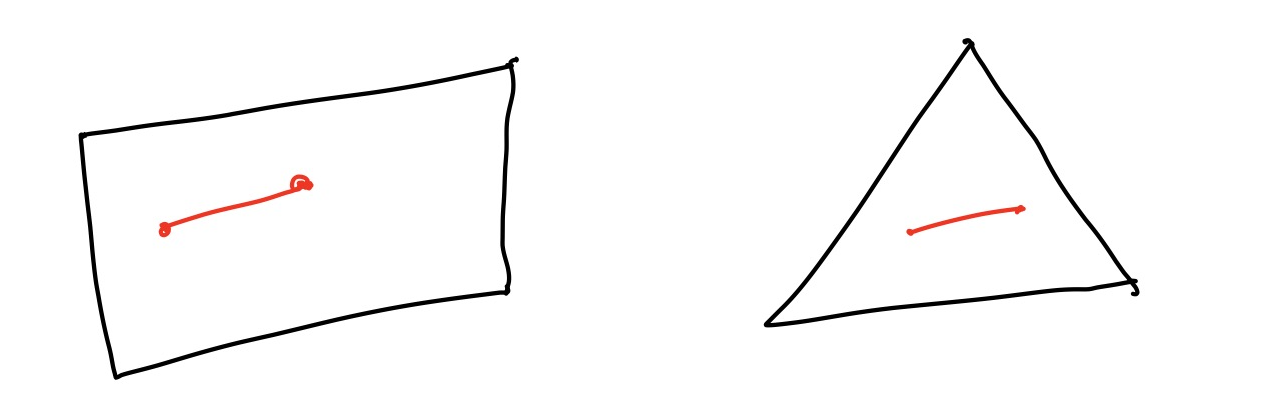
\includegraphics[scale=0.2]{convex.PNG}
\caption{Convex sets}
\label{fig:convex}
\end{figure}

\begin{figure}
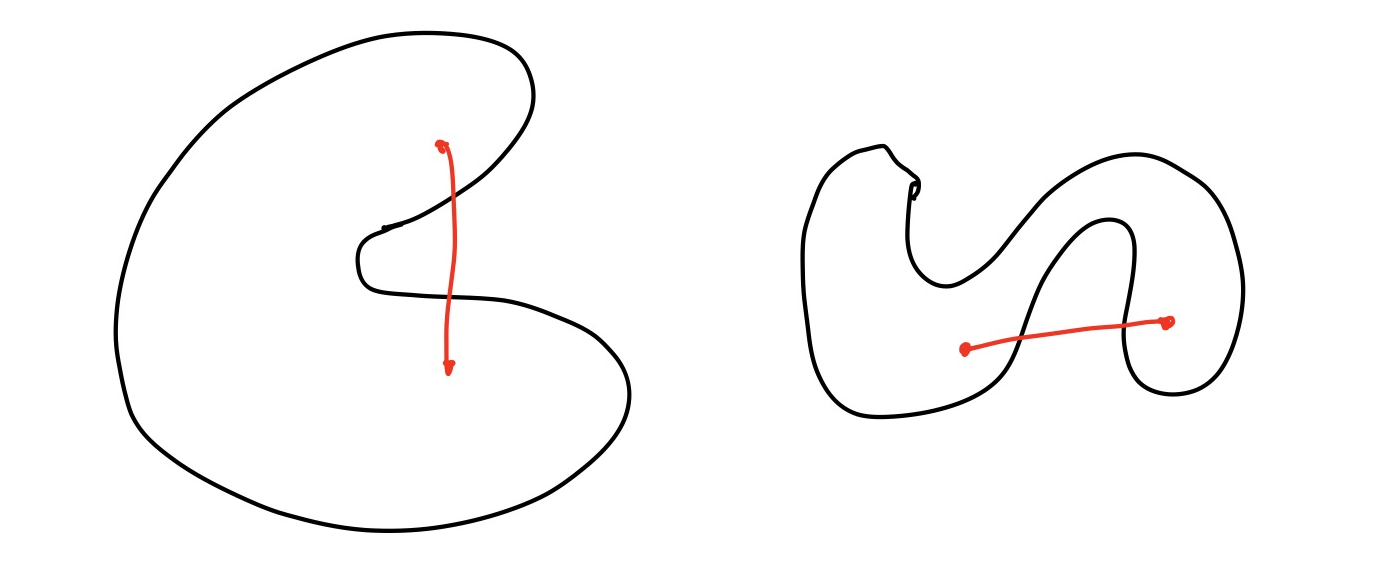
\includegraphics[scale=0.2]{notConvex.PNG}
\caption{Not convex sets}
\label{fig:notconvex}
\end{figure}

Here are some properties of convex sets (try proving them).
\begin{claim}
The following properties hold for convex sets.
\begin{enumerate}
\item Convex sets are closed under intersections.
\item A vector space is a convex set.
\end{enumerate}
\end{claim}

A vector $\vec x \in X$ is an \emph{extreme point} in the convex set $X$ if $\vec x$ cannot be represented as a convex combination of two other points in $X$.

The \emph{convex hull} of a set $X$ is the least convex set $Y$ which contains $X$ (that is $X \subseteq Y$).  For example, the convex hull of two points $\vec x, \vec y \in \Reals^2$ is the line segment joining $\vec x$ and $\vec y$. Figure \ref{fig:convexhull1} and \ref{fig:convexhull2} shows the convex hull of points $X$.
\begin{figure}
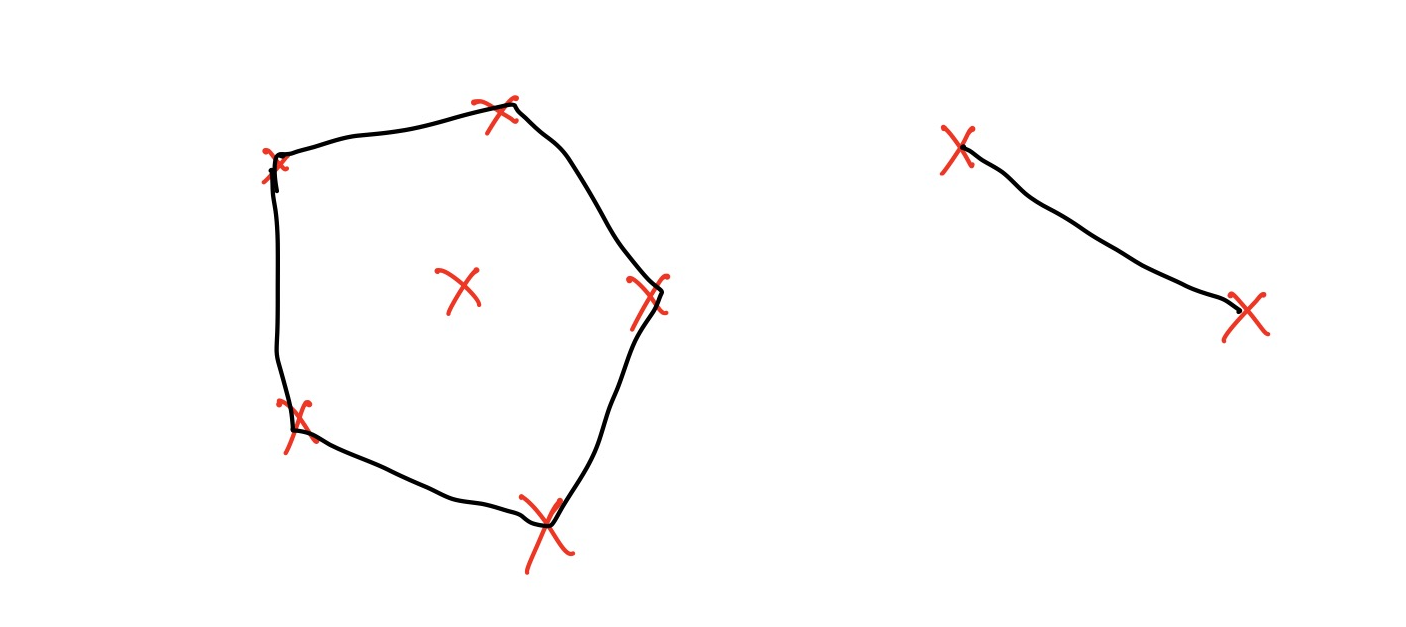
\includegraphics[scale=0.2]{convexHull.PNG}
\caption{Convex Hull of the red points.}
\label{fig:convexhull1}
\end{figure}
\begin{figure}
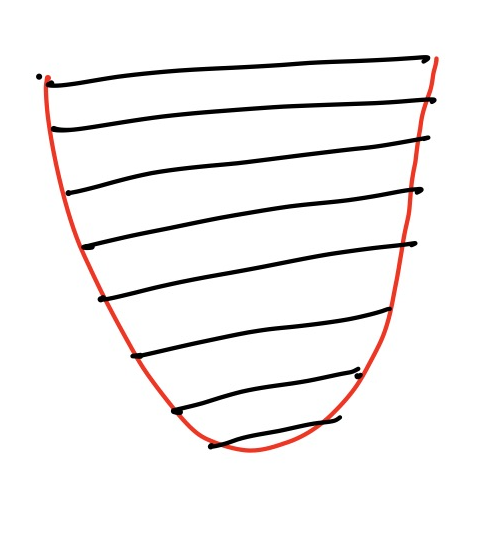
\includegraphics[scale=0.2]{convexHull2.PNG}
\caption{Convex Hull}
\label{fig:convexhull2}
\end{figure}


%\section{Standard form LP - geometric view}


\section{Canonical form LP - algebraic view}
Let $\mat{A'}$ be an $m \times n-m$ matrix. That is the matrix has $m$ rows and $n-m$ columns. Let $\vec c' \in \Reals^{n-m}$ be a real vector. Here we have $n \geq m$.

Consider the LP in standard form. Find an $x \in \Reals^{n-m}$ where  \lpstd{x'}{c'}{A'}{b}
This can be converted into an LP in canonical form as follows. For the $i^{th}$ in-equality constraint $\dotprod{a_i'}{x'} \leq  b_i$, we introduce a new variable $x_{n-m+i}$ and add the following constraints
\begin{align*}
\dotprod{a_i'}{x'} + x_{n-m+i} = b_i \\
x_{n-m+i} \geq 0
\end{align*}
This gives us the following LP in canonical form \lp{x}{c}{A}{b}
Here $\vec c \in \Rn$ and $\trans{\vec c} = (\trans{\vec c'},0,0,\dots,0)$ (This is an abuse of notation which means the last $m$ elements of the vector $\vec c$ are $0$s and the first elements correspond to that of $\vec c'$). The vector $\vec x \in \Rn$ and matrix $\mat{A}$ is of the following form.
\[
\mat{A} = \Matrix{ ,  ,,\vline, , , , , , ; , ,,\vline, , , , , , ;,\mat{A'}, ,\vline, , , \Imatrix, , , ; , ,,\vline, , , , , , ; , ,,\vline, , , , , , }
\]

The set of all feasible points (called the feasible set) of this LP in the canonical form is 
\[
F_C = \{\vec x \in \Rn \mid \mat A \vec x = \vec b \text{ and } \vec x \geq 0\}
\]
This set is closely related to the feasible set of the LP in standard form. We now describe a mapping $f: F_S \rightarrow F_C$. Let $\vec x' \in F_S$. Now consider the vector $\vec x \in \Rn$ where $x_j$ for a $j \leq n$ is given as
\[
x_{j} = \begin{cases}
x'_j \text{ if } j \leq n-m \\
b_i - \dotprod{a_i'}{x'} \text{ if } j = n-m+i \text{ and } i \leq m \\
\end{cases}
\]
The first claim is 
\begin{claim}
The above vector $\vec x$ belongs to $F_C$.
\end{claim}
\begin{proof}
This is an exercise.
\end{proof}
Therefore, the above mapping takes every vector $\vec x' \in F_S$ to a vector $\vec x \in F_C$. Let us represent this mapping by $f:F_S \rightarrow F_C$.	

\begin{claim}
Let $V \subseteq F_S$ be the set of extreme points in $F_S$. Then $f(V)$ is the set of extreme points in $F_C$.
\end{claim}
\begin{proof}
This is an exercise.
\end{proof}

We will now give an alternate (algebraic) definition of the extreme points of $F_C$. First a few definitions. For a vector $\vec x \in \Rn$ and a set $B \subseteq \{1,2,\dots,n\}$ we denote by $\vec{x}_{\overline B} = 0$ to mean $x_j = 0$ for all $j \notin B$. For example, consider $x = \trans{(2,3,0,0)} \in \Reals^4$. Then $x_{\overline{\{1,2\}}} = 0$ since $x_3=x_4 = 0$.

We say that $\vec x \in F_C$ is a \emph{basic feasible point}, if there exists a set $B \subseteq \{1,2,\dots,n\}$ such that the set of column vectors $\{A_j ~|~ j \in B\}$ form a basis for the column space of $\mat A$ (denoted by $\cspace{A}$) and $x_{\overline B} = 0$. In other words the vector $b$ is represented as a positive linear combinations of a basis of $\mat A$. The set of all basic feasible point is called \emph{basic feasible set} (\BFS for short).
\[
\BFS = \{\vec x \in F_C \mid \vec x \text{ is a basic feasible point.}\}
\]

The following assumption is going to be assumed henceforth.
\begin{mdframed}[backgroundcolor=light-gray, linecolor=light-gray]
{\bf Assumption I:} The rows of $\mat A$ are independent. Note that the number of rows is represented by $m$.
\begin{exercise}
Show that a basis for the column space of $\mat A$ has $m$ vectors.
\end{exercise}

\begin{exercise}
Given a matrix where rows are dependent, give an equivalent LP with independent rows.
\end{exercise}
\end{mdframed}

From the above assumption, we note that the number of non-zeros in a vector $\vec x \in \BFS$ is atmost $m$. The reason for at most $m$ and not exact $m$ is because it can happen that the co-efficient of a basis vector is also $0$. Therefore the number of zeros is atleast $n-m$. 

The next lemma is important.
\begin{lemma}
\label{lem:BFS}
The \BFS form the extreme points of $F_C$.
\end{lemma}
\begin{proof}
We need to show two directions for the proof. 

First we show that an extreme point of $F_C$ is a \BFS. 

We now show the other direction of the lemma. That is,  \BFS is an extreme point of $F_C$. This is left as an exercise.
\end{proof}

\BFS are the most important points in the LP. We will soon see that the optimum occurs at one of the \BFS.

\begin{mdframed}[backgroundcolor=light-gray, linecolor=light-gray]
{\bf Special Case:} The feasible set $F_C$ is bounded.

We say that a set $X \subseteq \Rn$ is \emph{bounded} if there exists an $M \in \Reals$ such that for all $\vec x \in X$, we have that $\vec x \leq M^n$. Convex sets which are closed and bounded satisfy a nice property.
\begin{claim}
Let $X$ be a closed bounded convex set. Then, $X$ is equal to the convex hull of its extreme points.
\end{claim}

Therefore, if $F_C$ is bounded, we have that the convex hull of \BFS gives us $F_C$. The following lemma captures the importance of \BFS in bounded sets. It says, if there is an optimal solution to the LP, then it occurs at one of the points in \BFS.
 
\begin{claim}
\label{claim:bounded}
Let the feasible set be bounded. If there is an optimal solution, then it occurs at a \BFS.
\end{claim}
\begin{proof}
Let $\vec x$ be an optimal solution. That is $
\rowvec{c} \vec x = \min \{\rowvec{c} \vec y \mid \vec y \in F_C\}$. In other words, 
\begin{equation}
\label{eq:optbound}
\forall \vec y \in F_C, ~\rowvec{c}\vec y \geq \rowvec{c} \vec x
\end{equation}
We show that there exists an $\vec x^* \in \BFS$ such that $\rowvec{c}{\vec x^*}= \rowvec{c}\vec x$. Let us assume $\vec x \notin \BFS$. From Lemma \ref{lem:BFS} we know that $\vec x$ is not an extreme points and hence can be written as a convex combination of vectors in $\vec z_i \in \BFS$ (using claim \ref{claim:bounded}). That is, $\vec x = \sum_{i=1}^k \lambda_i \vec z_i$ where $\sum_i \lambda_i = 1$. Let us assume without loss of generality, $\rowvec{c}\vec z_1 \leq \rowvec{c} \vec z_i$ for all $i \leq k$. Therefore 
\begin{equation}
\label{eq:opttwo}
\rowvec{c} \vec x \geq (\sum_{i=1}^k \lambda_i) ~\rowvec{c} \vec z_1 = \rowvec{c} \vec z_1
\end{equation}
From Equation \ref{eq:optbound} and \ref{eq:opttwo} we have that $\rowvec{c} \vec z_1 = \rowvec{c} \vec x$ and therefore $\vec z_1 \in \BFS$ is also an optimum point.
\end{proof}
\end{mdframed}

\section{Simplex algorithm}
With the intuition that the optimum occurs at one of the \BFS, our algorithm will be to check all the \BFS and return the optimal value. We have a better algorithm (which in the worst case is as bad as the naive algorithm) is very good in practise. The algorithm is called \emph{Simplex} and the fundamental idea is to start from a \BFS and keep going to a neighbouring vertex which is better in the objective function. Before we formally see the algorithm, let us define what are neighbouring \BFS.

We say that two basis $B, B' \subseteq \{A_1,A_2,\dots,A_n\}$ are \emph{neighbours} if $|B \cap B'| = m-1$. That is, they share exactly $m-1$ columns. Each has one column which is not in the other. We say that $\vec x, \vec y \in \BFS$ are \emph{neighbours} if there exists two basis $B, B'$ which are neighbours such that the basis associated with $\vec x$ and $\vec y$ are $B$ and $B'$ respectively. In other words, there are atleast $n-m-1$ locations where both $\vec x$ and $\vec y$ are zeros.

The Simplex algorithm is given in Algorithm \ref{alg:simplex}.

\begin{algorithm}
\caption{Simplex algorithm}
\label{alg:simplex}
\begin{algorithmic}
\STATE Find an initial \BFS $\vec x$
\WHILE{$\exists \vec y$ which is a neighbour of $\vec x$ and $\dotprod{c}{y} < \dotprod{c}{x}$}
	\STATE $\vec x = \vec y$
\ENDWHILE
\RETURN $\vec x$
\end{algorithmic}
\end{algorithm}

\subsection{Neighbouring \BFS}
Our first algorithmic challenge is to identify a neighbouring $\vec y \in \BFS$ given a $\vec x \in \BFS$ where $\dotprod{c}{y} < \dotprod{c}{x}$. That is, a neighbour whose cost is lesser that at $\vec x$. Let $B$ be the basis associated with vector $\vec x$ and $N$ the rest of the column vectors of $\mat{A}$. We can always re-arrange the columns so that the first $m$ columns is $B$. We also denote the various components of $\mat{A}, \vec x, \vec c$ as given below.
\[
\mat{A} = \Matrix{ , , , , \vline , , , ; , , , , \vline , , , ; , , \mat{A}_B , , \vline , , \mat{A}_N, ; , , , , \vline , , , ; , , , , \vline , , , }, \vec x = \Matrix{ ; \vec x_B; ; \hline;  \vec x_{N}}, \vec c = \Matrix{ ; \vec c_B; ; \hline;  \vec c_{N}}
\]
Therefore, we can write $\mat{A} \vec x = \vec b$ equivalently as $\mat{A}_B \vec x_B + \mat{A}_N \vec x_N = \vec b$ and the objective function as $\rowvec{c}\vec x = \rowvec{c}_B \vec x_B + \rowvec{c}_N \vec x_N$. Also note that $\vec x_N = 0^{n-m}$. 

Let $\vec x$ be a \BFS corresponding to basis $B$. Our plan is to find a basis $B'$ which is a neighbour to $B$. Let us consider that we want to include the column $A_j$ in $B'$. This would mean we will have to remove some other column from $B$. Without loss of generality, let us assume $B = \{A_1,A_2,\dots,A_m\}$ and $j>m$. Since $B$ forms a basis we have that there exists $\alpha_i$s such that
\begin{equation}
\label{eq:aj}
A_j = \sum_{i=1}^m \alpha_i A_i
\end{equation}

We also have that
\begin{equation}
\label{eq:b}
b = \sum_{i=1}^m x_i A_i
\end{equation}

\begin{mdframed}[backgroundcolor=light-gray, linecolor=light-gray]
Assumption: We will assume that $x_i > 0$ for all $i \leq m$. The tricky \emph{degenerate} case of some of $x_j=0$ is skipped in the lecture notes.
\end{mdframed}

Consider the following equation (we fix the $\theta$ later): Eq. \ref{eq:b} - $\theta$ Eq. \ref{eq:aj}.
\[
b = \sum_{i=1}^m (x_i - \theta \alpha_i) A_i + \theta A_j
\]

The neighbour \BFS to $\vec x$ is now given by $\vec y$ where $y_i$ is
\[
y_{i} = \begin{cases}
x_i - \theta \alpha_i \text{ if } i \leq m \\
\theta \text{ if } i = j \\
0 \text{ otherwise} \\
\end{cases}
\]

There are two cases to be considered now.

\noindent {\bf Case I:} There is atleast one $\alpha_i > 0$. In this case, take $\theta$ as follows
\[
\theta = min \{\frac{x_i}{\alpha_i} \mid \alpha_i > 0 \}
\]
Let $\theta = \frac{x_k}{\alpha_k}$. Then we have that $y_k = 0$ and all other $y_i \geq 0$. Moreover $\vec y$ is a \BFS with basis 
$B' = B \backslash \{A_k\} \cup \{A_j\}$. We can now check if $\dotprod{c}{y} < \dotprod{c}{x}$ and return $\vec y$ as a ``good'' neighbour if the cost decreases. Otherwise we find another neighbour and continue this procedure.

\noindent {\bf Case II:} All $\alpha_i \leq 0$. In this case $y_i$s increases as we increase $\theta$. We can therefore increase $y_i$ to as big a number as we want. Note that this cannot happen in a bounded $F_C$. On the other hand, we can look at the cost function $\dotprod{c}{y}$. It either increases as $\theta$ increase or decreases. If it is increasing, we are not interested we can skip and go to find another neighbour of $\vec x$. On the other hand, if it is decreasing, we can decrease $\dotprod{c}{y}$ to as much as we want and therefore, there is no optimum value. 

This gives an algorithm to find a neighbouring \BFS.

\subsection{Finding an initial \BFS}

\subsection{Correctness of Simplex algorithm}
Showing the following claim gives us the correctness of the Simplex algorithm.
\begin{theorem}
Let $\vec x$ be a \BFS such that for all neighbours $\vec y \in \BFS$ we have $\dotprod{c}{y} \geq \dotprod{c}{x}$. Then $\vec x$ is an optimal solution.
\end{theorem}
\begin{proof}
First we understand the relationship between $\vec x$ and its neighbours. Let $B$ be the basis of $\vec x$ and let $\vec z$ be a neighbour 
with basis $B' = B \backslash \{A_k\} \cup \{A_j\}$. We will use the matrix notation as given below.
\[
\mat{A} = \Matrix{ , , , , \vline , , , ; , , , , \vline , , , ; , , \mat{A}_B , , \vline , , \mat{A}_N, ; , , , , \vline , , , ; , , , , \vline , , , }, \vec x = \Matrix{ ; \vec x_B; ; \hline;  \vec x_{N}}, \vec c = \Matrix{ ; \vec c_B; ; \hline;  \vec c_{N}}
\]

Since $\vec x_{N} = \vec 0$, we have that $\mat{A}_B \vec{x}_B = b$. Since $A_j$ is in the basis for $\vec z$ we have that $\mat{A}_B \vec{z}_B + z_j A_j=b$. Subtracting, we have $\mat{A}_B \vec{x}_B - \mat{A}_B \vec{y}_B - z_j A_j = 0$. Therefore,
\begin{equation*}
\vec{x}_B - \vec{z}_B = z_j \mat{A}_B^{-1} A_j
\end{equation*}
Now let us calculate the cost difference at both the places
\[
0 \geq \dotprod{c}{x}-\dotprod{c}{y} = \rowvec{c}_B{(\vec x_B - \vec z_B)} - c_j z_j = z_j \rowvec{c}_B \mat{A}_B^{-1} A_j - c_j z_j
\]
Since $z_j > 0$ we have the inequality for all $j \notin B$.
\begin{equation}
\label{eq:loss}
c_j - \rowvec{c}_B \mat{A}_B^{-1} A_j  \geq 0
\end{equation}

Now we show that $\vec x$ is an optimal point. Assume not. Let $\vec y$ has a better objective value. That is,
$\rowvec{c}_B \vec{y}_B + \rowvec{c}_N \vec{y}_N =\dotprod{c}{y} < \dotprod{c}{x} = \rowvec{c}_B \vec{x}_B$.
Therefore,
\begin{equation}
\label{eq:costyb}
\rowvec{c}_B (\vec{y}_B - \vec{x}_B) + \sum_{j \notin B} c_j y_j < 0
\end{equation}

We know that $0 = \mat{A}(\vec y - \vec x) = \mat{A}_B (\vec y_B - \vec x_B) + \sum_{j \notin B} y_j A_j$. Therefore,
\begin{equation}
\label{eq:ybxb}
\vec y_B - \vec x_B = \sum_{j \notin B} - y_j \mat{A}_B^{-1} A_j
\end{equation}
We can substitute the above equation in Eq. \ref{eq:costyb} giving us
\[
\sum_{j \notin B} (c_j - \rowvec{c}_B \mat{A}_B^{-1} A_j) y_j < 0
\]
This gives us a contradiction from Eq. \ref{eq:loss} and since $y_j > 0$ ($y_j=0$ will not satisfy above inequality). 
\end{proof} 

\section{Matching using LP}
A \emph{bipartite graph} $G$ is represented by $G=(U,V,E)$ where $U \cup V$ are the set of vertices and edges are denoted by $E \subseteq U \times V$. A \emph{matching} $M \subseteq E$ of a bipartite graph $G$ is a set of edges such that for any vertex $v$ of $G$ at most one edge incident on $v$ is in $E$. In the \emph{maximal matching problem}, given a bipartite graph, we interested in finding out a matching of highest cardinality. We reduce the problem to an LP as follows. Without loss of generality we assume cardinality of $U$ is equal to cardinality of $V$ (otherwise add some vertices with no edges) which is equal to $n$. 

We introduce variables $x_{ij}$ for all $i \in U$ and $j \in V$. We want a solution to the LP where $x_{ij} \in \{0,1\}$ for all $i$ and $j$. We can view any assignment of $x_{ij}$s to $\{0,1\}$ as a set of edges $X = \{(i,j) \in E \mid x_{ij}=1\}$. Consider the following LP.

\begin{align*}
\maximize ~\sum_{(i,j) \in E} x_{ij} \\
\forall i \in U, \sum_{j \in V} x_{ij}=1 \\
\forall j \in V, \sum_{i \in U} x_{ij}=1 \\
\forall i,j, 0 \leq x_{ij} \leq 1 
\end{align*}

Unfortunately, the optimal solution to the LP may not have integer values for $x_{ij}$. The next claim shows that there is always an integer solution associated with a maximal matching.
\begin{claim}
If $M \subseteq U \times V$ is a maximal matching, then there is an optimal solution with integer values and where $x_{ij}=1$ for all $(i,j) \in M$.
\end{claim}
\begin{proof}
We give the assignment to $x_{ij}$s as follows. Let $\{u_1, u_2, \dots, u_k \} \subseteq U$ and $\{v_1, v_2, \dots, v_k \} \subseteq V$  be the set of vertices not matched in $M$. For the feasible point, make $x_{u_i v_i} = 1$. Note that, there is no edge between $(u_i,v_i)$. Otherwise this would have been in the maximal matching.
\end{proof}

It is also easy to see that if we have an integer optimal solution, then we have a maximal matching. Now, we come to deal with the non-integer solution problem. We show that if we have a non-integer solution we can get one out of that. In practise this wont be necessary though. It is worth noting that due to some properties of the linear constraints in the maximal matching LP, the optimal solution is always integral (we skip this linear algebraic argument here). We give a method to extract an integer solution of same optimal value from a rational optimal solution.

Let there be $K$ number of fractions in the solution. We reduce the number of fractions atleast by one without changing the optimal condition. Let $u \in U$ be a vertex where there is an edge with fractional value, say $(u,v)$. Take that edge. This means that $v$ has another edge which is also fractional. We take that edge leading to another vertex having another fractional edge. We continue doing this until we hit upon a cycle. Let us concentrate on the cycle. Assume the cycle starts from $u \in U$. We subtract $\theta$ (a very very small value) from $x_{uv}$ (we assume $(u,v)$ is the edge in the cycle) and add $\theta$ on the other edge starting from $v$ in the cycle.  This is continued. That is, for every edge from $U$ to $V$ we subtract $\theta$ whereas we add $\theta$ in the other direction. Note that $\theta$ is smaller than all $x_ij$s in the cycle.

\begin{claim}
The optimal value of the LP does not change on this new assignment.
\end{claim}
\begin{proof}
Let us assume that the optimal value increases. A contradiction since $x$ is an optimal solution and therefore we cannot increase the optimal value. So, let us assume that the optimal value decreases. Then, consider an alternate assignment where we replace $\theta$ by $-\theta$. Due to the previous reason, the optimal value should now increase. This leads to another contradiction.
\end{proof}

We can therefore take a $\theta$ such that one of $x_{ij}$s becomes an integer solution (either $0$ or $1$) and the rest remains inside the feasible region. This reduces the number of fractional solutions by atleast one. Continuing the process will lead to an optimal solution with all integer values.

%\printindex

%\bibliography{papers}
%\bibliographystyle{plain}
\end{document}
